% !TeX spellcheck = en_GB
\documentclass[
 paper=A4,pagesize=automedia,fontsize=12pt,
 BCOR=15mm,DIV=22,
 twoside,headinclude,footinclude=false,
 fleqn,                     % fleqn = linksbündige Ausrichtung von Formeln
 bibtotocnumbered,          % Literaturverz. im Inhaltsverz. eintragen
 liststotoc,                % Abbildungsverz. im Inhaltsverz. eintragen
 listsleft,                 % Abbildungsverz. an der längsten Nummer ausrichten
 %pointlessnumbers,          % kein Punkt nach Überschriftsnummerierung
 cleardoublepage=empty      % Vakatseiten ohne Paginierung
]{scrbook}
\setlength\parindent{0em}

% Kodierung, Schrift und Sprache auswählen
\usepackage[utf8]{inputenc}
\usepackage[T1]{fontenc}
\usepackage{babel}
% damit man Text aus dem PDF korrekt rauskopieren kann
\usepackage{cmap}
% Layout: Kopf-/Fußzeilen, anderthalbfacher Zeilenabstand
\usepackage{scrpage2} \pagestyle{scrheadings}
                      \clearscrheadfoot
                      \ihead{\headmark}\ohead{\pagemark}
                      \automark[subsection]{section}
                      \setheadsepline{0.5pt}
\usepackage{setspace} \onehalfspacing
\deffootnote{1em}{1em}{\textsuperscript{\thefootnotemark }}
% Grafiken, Tabellen, Mathematikumgebungen
\usepackage{graphicx,xcolor}
\usepackage{tabularx}
\usepackage{amsmath,amsfonts,amssymb}
% Darstellung von Fließumgebungen
\usepackage{flafter,afterpage}
\usepackage[section]{placeins}
\usepackage[margin=8mm,font=small,labelfont=bf,format=plain]{caption}
\usepackage[margin=8mm,font=small,labelfont=bf,format=plain]{subcaption}

\numberwithin{equation}{chapter}
\numberwithin{figure}{chapter}
\numberwithin{table}{chapter}

%%%%%%%%%%%%%%%%%%%%%%%%%%%%%%%%%%%%%%%%%%%%%%%%%%%%%%%%%%%%%%%%%%%%%%%%%%%%%%%%
% Ab hier ist Platz für eigene Ergänzungen (Pakete, Befehle, etc.)

% Dieses Paket liefert den Blindtext, der als Platzhalter in den Beispieldateien steht.
% Das kannst Du also entfernen, wenn Du den Blindtext nicht mehr brauchst.
\usepackage{lipsum}
%\usepackage{ bbold }
\usepackage{physics}
\usepackage{svg}
\usepackage{yfonts}
\usepackage{dsfont}
\usepackage{caption}
\usepackage{subcaption}
\usepackage[hidelinks]{hyperref}
\usepackage{multirow}
\begin{document}

\frontmatter


% Titelpageseite
\begin{titlepage}
 \begin{tabularx}{\linewidth}{X}
  \includegraphics[width=6cm]{TU_Logo_SW} \\\hline\hline

  \vspace{4.5em}

  \begin{singlespace}\begin{center}\bfseries\Huge
  
  Title of Bachelor thesis
  
  \end{center}\end{singlespace}

  \vspace{5.5em}

  \begin{singlespace}\begin{center}\large
   Bachelor-Arbeit \\ zur Erlangung des Hochschulgrades \\ 
   Bachelor of Science \\ 
   im Bachelor-Studiengang Physik
  \end{center}\end{singlespace}\medskip

  \begin{center}vorgelegt von\end{center}
  \begin{center}
   {\large Felix Soest} \\ geboren am 16.09.1998 in Düsseldorf
  \end{center}\medskip

  \begin{singlespace}\begin{center}\large
   Institut für Theoretische Physik \\
   Fakultät Physik \\
   Bereich Mathematik und Naturwissenschaften \\
   Technische Universität Dresden \\ 2021
  \end{center}\end{singlespace}
 \end{tabularx}
\end{titlepage}


% Gutachterseite
\thispagestyle{empty}\vspace*{48em}

Eingereicht am xx.~Monat~20xx\vspace{1.5em}
\par{\large\begin{tabular}{ll}
 1. Gutachter: & Prof.~Dr.~Walter~Strunz \\
 2. Gutachter: & Prof.~Dr.~Oscar~Dahlsten \\
\end{tabular}}


% Abstractseite
\newpage
\begin{center}\large\bfseries Summary\end{center}


Abstract \\ 
English: \\
Aufmerksamkeit
große Fragen?
unsere Frage
unsere Antwort

\vspace{20em}
Abstract \\ 
Deutsch \\
 
 
% Inhaltsverzeichnis
%\cleardoublepage
\tableofcontents



% Hauptteil
\mainmatter

\chapter{Introduction}
\lipsum
\section{Intro}
% !TeX root = ../BA_main_englisch.tex
% !TeX spellcheck = en_GB
Energy harvesting 

Due to the increasing availability of data, machine learning methods have become a standard approach in many fields such as natural language processing \cite{DBLP:journals/corr/VaswaniSPUJGKP17}.
Additionally, these methods are being applied to a broad range of problems in the physical sciences, from statistical physics to quantum computing \cite{Carleo_2019, wise2021using}.

Machine learning has also found use in the field of energy harvesting, concerned with extracting energy from external excitations, e.g. vibrations in human motion \cite{Liu2019}.


The remainder of this work is structured as follows.
In Section \ref{background} we review the collision model framework used in our approach and introduce two machine learning architectures.
We investigate the system under consideration in Section \ref{dep_dt} and apply the aforementioned architectures in Sections \ref{n_2_ml} to \ref{work_cost}.
We summarise our findings and provide an outlook in Section \ref{outlook}.

\chapter{Background}
\section{Supervised Machine Learning} \label{sml}
Machine learning is a subfield of artificial intelligence, `concerned with the question of how to construct computer programs that automatically improve with experience.' \cite{Mitchell97}
Supervised machine learning is one of the three machine learning disciplines, besides unsupervised and reinforcement learning.
The goal is to find a mapping between an input and an output, in our case an excitation and its respective optimal harvesting policy.
Multiple algorithms to find such a mapping exist, however for high dimensional problems artificial neural networks (ANNs) are usually used.
In the following sections we review two ANN architectures, the fully-connected feedforward ANN and the Long Short-Term Memory (LSTM) network.

\subsection{Fully-connected feedforward ANNs}
In this section we review ANNs, following the exposition given in \cite{lu2020dying}.
Let $\textfrak{N}$ be a fully-connected feedforward ANN, meaning there are no loops in the neuron connections and all neurons in a layer are connected to every neuron of the next layer, $\textfrak{N}: \mathbb{R}^{n_1} \to \mathbb{R}^{n_L}$. $n_1$ and $n_L$ denote the dimensionality of the input and output respectively. 
$\textfrak{N}$ has $L$ layers, or columns of neurons.
The network architecture is given by the amount of neurons $n_l$ in each hidden layer $l \in [2, L - 1]$ (see figure \ref{nn}).
The neurons in layer $l$ are represented by their activations $\vec{a}_l \in \mathbb{R}^{n_l}$, which represent the matrix multiplication output. Additionally each layer includes trainable parameters $W_l \in \mathbb{R}^{n_{l+1} \times n_{l}}$ and $\vec{b}_l \in \mathbb{R}^{n_l}$ called weights and biases respectively.
The activations can then be calculated using the following formulae \cite{TN_libero_mab2)53517}:
\begin{align*}
	\vec{a}_2 & = W_1 \vec{a}_1 + \vec{b}_1, \\
	\vec{a}_l & = W_{l-1} \xi(\vec{a}_{l-1}) + \vec{b}_{l-1}, \ l \in [3, L],
\end{align*}
where $\xi(x)$ is a function called the activation function applied elementwise. Historically, functions such as $\tanh$ and sigmoid have been used. However, it has been shown \cite{Maas2013RectifierNI, krizhevsky} that the rectified linear unit $\mathrm{ReLU}(x) = \mathrm{max}(0, x)$ often provides better results and is used here.

\begin{figure}
	\centering
	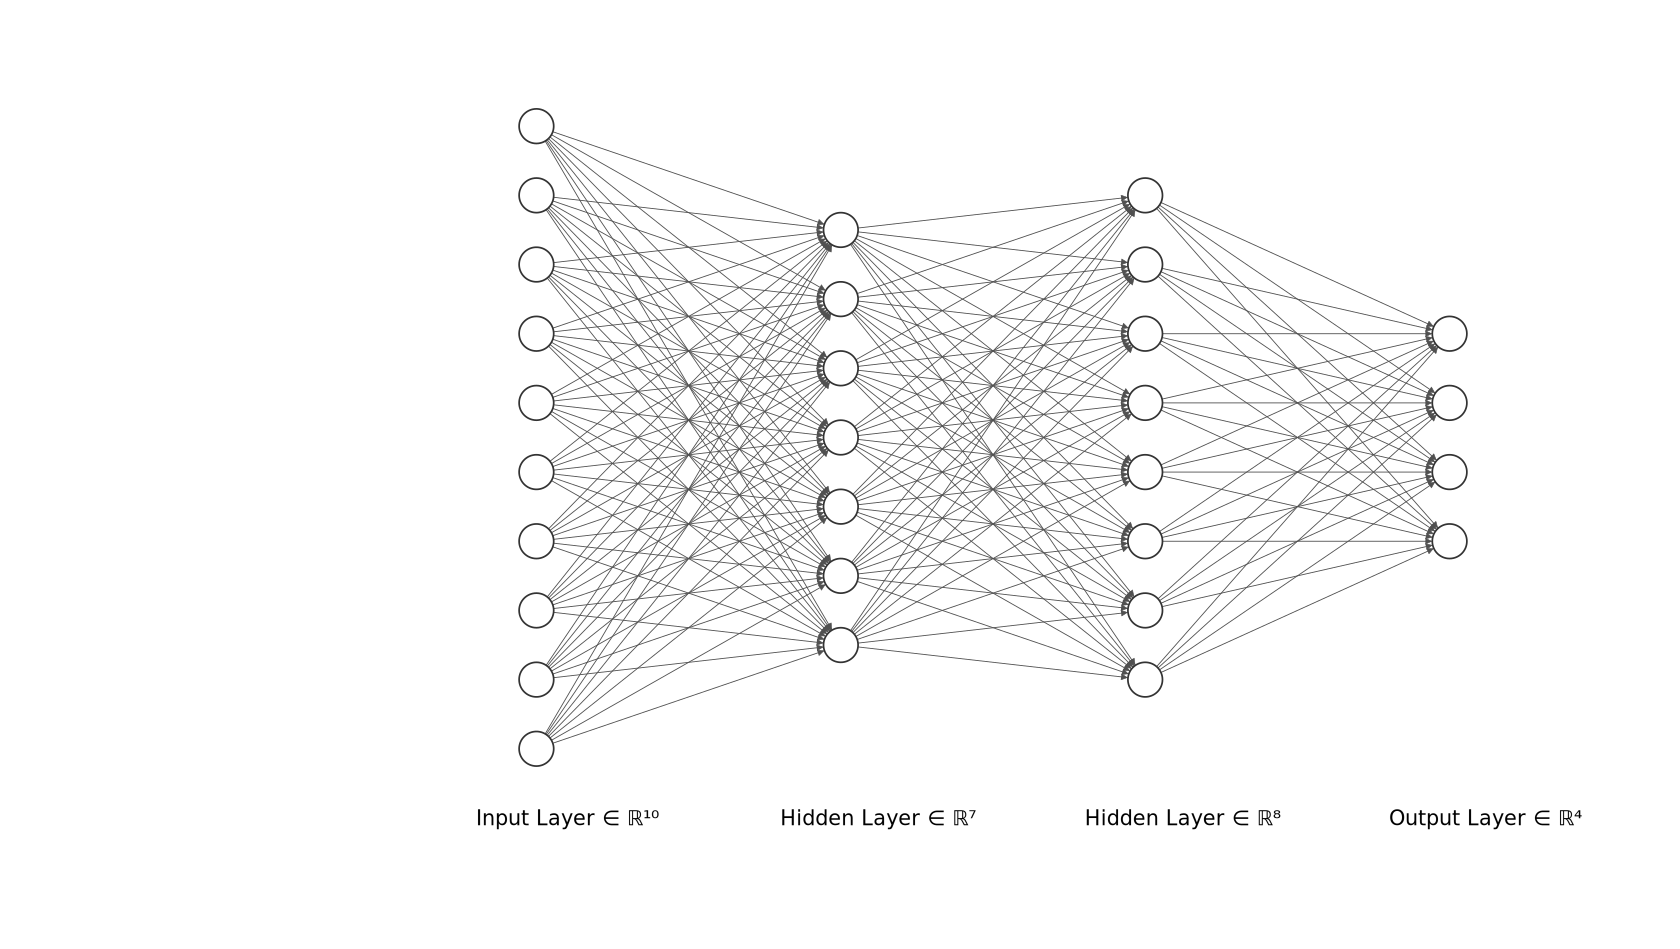
\includegraphics[width=0.6\textwidth]{img/nn}
	\caption{Example fully-connected feedforward ANN with four layers, including input, output and two hidden layers \cite{LeNail2019}.}
	\label{nn}
\end{figure}

\subsection{Long Short-Term Memory}
While the network architecture introduced in the previous section performs reasonably well on many problems, it destroys spatial and temporal correlations present in the data. 
Instead convolutional and recurrent networks are often used for these purposes, e.g. in image recognition and time series forecasting \cite{rumelhart1986learning, 10.1007/978-3-642-46466-9_18}.

Here we use the LSTM architecture, a type of recurrent neural network (RNN) introduced in \cite{doi:10.1162/neco.1997.9.8.1735}. 
The core idea of RNNs is the usage of loops to store and propagate information through time (figure \ref{rnn}).

\begin{figure}
	\centering
	\includegraphics[width=0.6\textwidth]{img/rnn}
	\caption{Example RNN with LSTM architecture. Each LSTM block has the same parameters and information is fed into the network sequentially.}
	\label{rnn}
\end{figure}

The network is made up of a row of LSTM cells which share parameters.
The cell uses the current input $x_t$ as well as the previous cell state $c_{t-1}$ and output $h_{t-1}$ to compute the output $h_t$.
Internally, the cell is comprised of multiple gates which control the storage of information, $i_t, f_t, g_t, o_t$, which are the input, forget, cell and output gates respectively.
The output and gates of each cell are computed using the following equations \cite{NEURIPS2019_9015}:
\begin{align*}
i_t & = \sigma (W_{ii} x_t + b_{ii} + W_{hi} h_{t-1} + b_{hi}), \\
f_t & = \sigma (W_{if} x_t + b_{if} + W_{hf} h_{t-1} + b_{hf}), \\
g_t & = \tanh (W_{ig} x_t + b_{ig} + W_{hg} h_{t-1} + b_{hg}), \\ 
o_t & = \sigma (W_{io} x_t + b_{io} + W_{ho} h_{t-1} + b_{ho}), \\
c_t & = f_t \odot c_{t-1} + i_t \odot g_t, \\
h_t & = o_t \odot \tanh (c_t),
\end{align*}
where $\odot$ is the Hadamard product and $\sigma(x)$ is the sigmoid function.
The input and forget gates $i_t, f_t$ express to what extent new data should be incorporated or deleted from the current cell state $c_t$ respectively.

\begin{figure}
	\centering
	\includegraphics[width=0.6\textwidth]{img/lstm}
	\caption{Visualisation of a single LSTM cell. The input $x_t$ enters the cell in the bottom left and is concatenated with the output $h_{t\text{-}1}$ of the previous cell. The combined data then enters multiple single-layer neural networks represented by orange rectangles with their respective activation function. The forget gate $f_t$ removes data from the previous cell state $c_{t\text{-}1}$ while $i_t$ and $g_t$ control how new data is added to the memory. $\tanh$ is applied elementwise over the cell state (yellow ellipse) to determine the cell output $h_t$ together with the output gate $o_t$.}
	\label{lstm}
\end{figure}

\subsection{Training \& Backpropagation}
To train an ANN a cost function is defined, often the mean squared error 
\begin{align*}
	\mathrm{MSE} = \frac{1}{N} \sum_{i=1}^N (\vec{a}_{L, i} - \vec{y}_i)^2,
\end{align*}
where the summation is performed over the training data $\{(\vec{x}_i, \vec{y}_i)\}$ with $N$ samples. $\{\vec{x_i}\}$ is the input, $\{\vec{y_i}\}$ the output data and $\vec{a}_{L, i} = \textfrak{N}(\vec{x}_i)$ the output of the neural network.
The so-called backpropagation algorithm is used to calculate the gradient of the cost function with respect to the trainable parameters and improve the performance of the ANN \cite{rumelhart1986learning, nielsenneural}.



\section{Collision model dynamics} \label{col_model}
A standard approach to modeling open quantum systems is the collision model.
The system under consideration interacts with a series of ancilla systems through a unitary transformation on the combined system-ancilla state \cite{Lorenzo_2017}. After a short interaction time $\Delta t$, the ancilla systems are traced out to receive the system state.
This type of interaction will in general lead to entanglement between system and ancilla.
To ensure the ancilla and system states remain pure, we follow the approach used in \cite{beyer2020}.
The interaction between ancillas and system is modelled by partial scalar products, leading to von-Neumann dynamics on the system in the continuous limit.

\section{Setting}
%In the following we use a three qubit system, which we call Drive, System and Transducer. The interaction is given by the Hamiltonian
$H_{DST} = $
\lipsum


\chapter{Experimental Results}
%In the following section we present our findings.
The training data is created using a minimisation algorithm \cite{2020SciPy-NMeth}, which finds the optimal Transducer protocol $\{|\psi_T^i \rangle\}$ given a Drive sequence $\{|\psi_D^i \rangle\}$.
The networks are trained to learn the mapping $\{|\psi_D^i \rangle\} \to \{|\psi_T^i \rangle\}$.
Both the input (Drive) and output (Transducer) are transformed by the embedding
\begin{align*}
	\left\{
	\begin{pmatrix}
	\theta^i & \phi^i \\
	\end{pmatrix}
	\right\}
	\to
	\left\{
	\begin{pmatrix}
	sin(\theta^i) & cos(\theta^i) & sin(\phi^i) & cos(\phi^i) \\
	\end{pmatrix}
	\right\}.
\end{align*}
The reasons for this operation are twofold: it normalises the data to the interval $[-1, 1]$, which is beneficial to learning \cite{LeCun2012}. Additionally it adds information regarding the periodicity of the qubit angle representation.


To compare the accuracy of different models a performance indicator is required. 
Naturally one might use the MSE as introduced in section \ref{sml}.
Instead we define the \textit{efficiency} of a model $\textfrak{N}$ on a dataset $\{(\vec{x}_i, \vec{y}_i)\}$ as
\begin{align}
	\eta = \frac{1}{N} \sum_{i=1}^N \frac{W(\vec{x}_i,\textfrak{N}(\vec{x}_i))}{W(\vec{x}_i,\vec{y}_i)},
\end{align}
i.e. the arithmetic mean of the ratios of work output predicted by the model to optimal work output.
The function $W(\vec{x}_i, \vec{y}_i) = W(\{\ket{\psi_D}\}_i, \{\ket{\psi_T}\}_i)$ returns the work given a Drive and Transducer protocol.
\section{Dependence of $\Delta \mathrm{T}$ on Work Output}
We start our investigation by determining the work output $W$ when varying the time between qubit switching $\Delta t$.
If the System qubit is initialised in the pure state $\rho_S = \ket{0} \bra{0}$, the work output for a single jump is given by (see appendix \ref{deriv_jump} for a derivation)
\begin{equation} \label{single_work}
	W = \frac{1}{\abs{\alpha}} sin(2\abs{\alpha}\Delta t) \Im{(\tau' - \tau) \alpha^*}
\end{equation}
\begin{equation*}
	\alpha = \frac{1}{2} \left[sin(\theta_D^1) e^{i\phi_D^1} + sin(\theta_T^1) e^{i\phi_T^1}\right], \\
	\tau' - \tau = \frac{1}{2} \left[ sin(\theta_T^2)e^{i\phi_T^2} - sin(\theta_T^1)e^{i\phi_T^1} \right].
\end{equation*}

From equation \ref{single_work} it becomes evident that for $\Delta t \to 0, W \to 0$. This is confirmed by the following where, for multiple values of $N$, we simulate 500 random Drive functions for each $\Delta t$ and find their optimal Transducer policy. The average work output over the 500 runs scaled by the amount of PWC steps $\overline{W}/N$ for 20 values of $\Delta t$ is shown in figure \ref{dt_dep}.

\begin{figure}
	\centering
	\includegraphics[width=0.7\textwidth]{img/dt_dep}
	\caption{We plot the average work $\overline{W}$ over 500 runs for random excitations divided by amount of PWC steps $N$, for all of which we use $\rho_0 = \ket{0}\bra{0}$. The error bars correspond to the standard deviation $\sigma_{\overline{W}}$.}
	\label{dt_dep}
\end{figure}
\section{$N=2$: Learning Single Jump Optimal Control Sequences}
% !TeX spellcheck = en_GB
For the simplest case of $N = 2$, we generate data sets for $\rho_0 = \ket{0} \bra{0}, \ket{+} \bra{+}$ and random pure states.
We train each data set on a fully-connected feedforward ANN with a single hidden layer with 10 neurons.
The efficiency of the models is presented in Table \ref{n2efftable}.
For $N = 2$, starting in an eigenstate of the drive Hamiltonian $H_{DS}$ gives the highest model efficiency, as the optimal transducer policy is trivial to learn and implement (see Appendix \ref{n2_opt_pol}).

For random initial states the efficiency is close to zero.
This is to be expected, as without knowledge of the system state $\rho_0$ the optimal transducer policy cannot be determined.\footnote{The deviation from zero is a relic of the finite sample size. For $N_{\mathrm{data}} \to \infty$ it would disappear.}
For comparison, we train a network with the same hyperparameters using the random initial state as additional inputs.
This increases the test data efficiency, but is still far below the efficiency for $\rho_0 = \ket{+} \bra{+}$.


\begin{table}[h]
	\centering
	\begin{tabular}{ c | c }
		$\rho_0$ & $\eta_{test} \ [\%]$ \\
		\hline
		$\ket{0} \bra{0}$ & 72.7 \\
		$\ket{+} \bra{+}$ & 100.0 \\
		Random & 0.5 \\
		Random, $\rho_0$ as input & 43.0 \\
	\end{tabular}
	\caption{Efficiencies $\eta$ on the test data for models with a single hidden layer with 10 neurons trained on drive protocols with $N = 2$ and differing initial states $\rho_0$.}
	\label{n2efftable}
\end{table}

\chapter{Summary and Outlook}


\appendix
\chapter{Derivations}
\section{Single jump work output}
\label{deriv_jump}
%\begin{align*}
%	H_S(\theta_D(t), \phi_D(t), \theta_T(t), \phi_T(t)) = \frac{1}{2} \left[sin(\theta_D(t)) e^{i\phi_D(t)} + \sin(\theta_T(t)) e^{i\phi_T(t)}\right] \sigma_{+} + h.c. \\
%	= \alpha \sigma_{+} + h.c. \\
%	\rho_S(t+1) = U \rho_S(t) U^\dagger, U = e^{-iH_S(t) \Delta \mathrm{T}} \\
%	dW(t) = -\textrm{Tr} \ \rho(t) dH \\
%	dH = H_S(\theta_D(t), \phi_D(t), \theta_T(t+1), \phi_T(t+1)) - H_S(\theta_D(t), \phi_D(t), \theta_T(t), \phi_T(t)) \\
%	= \frac{1}{2}(sin(\theta_T(t+1))e^{i\phi_T(t+1)} - \sin(\theta_T(t))e^{i\phi_T(t)}) \sigma_{+} + h.c. =: (\tau' - \tau) \sigma_{+} + h.c. \\
%	\textrm{For N=2 only one jump, analytical solution is possible:} \\
%	U = e^{-iH_S \Delta \mathrm{T}} = 
%	exp \begin{pmatrix}
%	0 & -i\alpha^* \Delta \mathrm{T} \\
%	-i \alpha \Delta \mathrm{T} & 0 \\
%	\end{pmatrix} = 
%	\frac{1}{2} \begin{pmatrix}
%	\frac{\alpha^*}{\abs{\alpha}} & -\frac{\alpha^*}{\abs{\alpha}} \\
%	1 & 1 \\
%	\end{pmatrix}
%	\begin{pmatrix}
%	e^{-i\abs{\alpha} \Delta \mathrm{T}} & 0 \\
%	0 & e^{i\abs{\alpha} \Delta \mathrm{T}} \\
%	\end{pmatrix}
%	\begin{pmatrix}
%	\frac{\abs{\alpha}}{\alpha^*} & 1 \\
%	-\frac{\abs{\alpha}}{\alpha^*} & 1 \\
%	\end{pmatrix} \\
%	= \begin{pmatrix}
%	cos(\abs{\alpha}\Delta \mathrm{T}) & -i\frac{\alpha^*}{\abs{\alpha}} \sin(\abs{\alpha}\Delta \mathrm{T}) \\
%	-i\frac{\abs{\alpha}}{\alpha^*} \sin(\abs{\alpha}\Delta \mathrm{T}) & \cos(\abs{\alpha} \Delta \mathrm{T}) \\
%	\end{pmatrix} \\
%	\mathrm{With} \ \rho_0 = \ket{0}\bra{0}, \mathrm{the \ time \ evolved \ state} \ \rho = U \rho_0 U^\dagger \mathrm{is} \\
%	\rho = \begin{pmatrix}
%	cos^2(\abs{\alpha} \Delta \mathrm{T}) & i\frac{\abs{\alpha}}{2\alpha} \sin(2\abs{\alpha} \Delta \mathrm{T}) \\
%	-i\frac{\abs{\alpha}}{2\alpha^*} \sin(2\abs{\alpha} \Delta \mathrm{T}) & \sin^2(\abs{\alpha} \Delta \mathrm{T})
%	\end{pmatrix} \\
%	W = -\mathrm{Tr} \begin{pmatrix}
%	0 & \tau'^* - \tau^* \\
%	\tau' - \tau & 0 \\
%	\end{pmatrix}
%	\begin{pmatrix}
%	cos^2(\abs{\alpha} \Delta \mathrm{T}) & i\frac{\abs{\alpha}}{2\alpha} \sin(2\abs{\alpha} \Delta \mathrm{T}) \\
%	-i\frac{\abs{\alpha}}{2\alpha^*} \sin(2\abs{\alpha} \Delta \mathrm{T}) & \sin^2(\abs{\alpha} \Delta \mathrm{T})
%	\end{pmatrix} \\
%	= \frac{1}{\abs{\alpha}} \sin(2\abs{\alpha}\Delta \mathrm{T}) \Im{(\tau' - \tau) \alpha^*}
%\end{align*}

\begin{align*}
	H_S(\theta_D(t), \phi_D(t), \theta_T(t), \phi_T(t)) = \frac{1}{2} \left[\sin(\theta_D(t)) e^{i\phi_D(t)} + \sin(\theta_T(t)) e^{i\phi_T(t)}\right] \sigma_{+} + h.c. \\
	= \alpha \sigma_{+} + h.c. \\
	dH = H_S(\theta_D(t), \phi_D(t), \theta_T(t+1), \phi_T(t+1)) - H_S(\theta_D(t), \phi_D(t), \theta_T(t), \phi_T(t)) \\
	= \frac{1}{2}(\sin(\theta_T(t+1))e^{i\phi_T(t+1)} - \sin(\theta_T(t))e^{i\phi_T(t)}) \sigma_{+} + h.c. =: (\tau' - \tau) \sigma_{+} + h.c. \\
	U = e^{-iH_S \Delta \mathrm{T}} = 
	exp \begin{pmatrix}
	0 & -i\alpha^* \Delta \mathrm{T} \\
	-i \alpha \Delta \mathrm{T} & 0 \\
	\end{pmatrix} = 
	\frac{1}{2} \begin{pmatrix}
	\frac{\alpha^*}{\abs{\alpha}} & -\frac{\alpha^*}{\abs{\alpha}} \\
	1 & 1 \\
	\end{pmatrix}
	\begin{pmatrix}
	e^{-i\abs{\alpha} \Delta \mathrm{T}} & 0 \\
	0 & e^{i\abs{\alpha} \Delta \mathrm{T}} \\
	\end{pmatrix}
	\begin{pmatrix}
	\frac{\abs{\alpha}}{\alpha^*} & 1 \\
	-\frac{\abs{\alpha}}{\alpha^*} & 1 \\
	\end{pmatrix} \\
	= \begin{pmatrix}
	\cos(\abs{\alpha}\Delta \mathrm{T}) & -i\frac{\alpha^*}{\abs{\alpha}} \sin(\abs{\alpha}\Delta \mathrm{T}) \\
	-i\frac{\abs{\alpha}}{\alpha^*} \sin(\abs{\alpha}\Delta \mathrm{T}) & \cos(\abs{\alpha} \Delta \mathrm{T}) \\
	\end{pmatrix} \\
	\mathrm{With} \ \ket{\psi_0} = a \ket{0} + b \ket{1}, \abs{a}^2 + \abs{b}^2 = 1, \ \mathrm{we \ have} \\
	\rho_0 = \begin{pmatrix}
	\abs{a}^2 & a b ^* \\
	a^* b & \abs{b}^2 \\
	\end{pmatrix}, \ \rho = U \rho_0 U^\dagger = \\
	\tiny
	\begin{pmatrix}
	\abs{a}^2 \ \cos^2(\abs{\alpha} \Delta \mathrm{T}) + \abs{b}^2 \ \sin^2(\abs{\alpha} \Delta \mathrm{T}) - \frac{1}{\abs{\alpha}} \sin(2 \abs{\alpha} \Delta \mathrm{T}) \Im{a b^* \alpha} & 
	\frac{\alpha^*}{2 \abs{\alpha}} i \ \sin(2 \abs{\alpha} \Delta \mathrm{T}) (\abs{a}^2 - \abs{b}^2) + \frac{\alpha^*}{\alpha} a^* b \sin^2(\abs{\alpha} \Delta \mathrm{T}) + a b^* \ \cos^2(\abs{\alpha} \Delta \mathrm{T}) \\
	\frac{\abs{\alpha}}{2 \alpha^*} i \ \sin(2 \abs{\alpha} \Delta \mathrm{T}) (\abs{b}^2 - \abs{a}^2) + \frac{\alpha}{\alpha^*} a b^* \ \sin^2(\abs{\alpha} \Delta \mathrm{T}) + a^* b \ \cos^2(\abs{\alpha} \Delta \mathrm{T}) & 
	\abs{a}^2 \ \sin^2(\abs{\alpha} \Delta \mathrm{T}) + \abs{b}^2 \ \cos^2(\abs{\alpha} \Delta \mathrm{T}) + \frac{1}{\abs{\alpha}} \sin(2 \abs{\alpha} \Delta \mathrm{T}) \Im{a b^* \alpha}
	\end{pmatrix} \\
	\mathrm{dW} = - \mathrm{Tr} \ \rho \ \mathrm{dH} = \frac{\abs{a}^2 - \abs{b}^2}{\abs{\alpha}} \sin(2 \abs{\alpha} \Delta \mathrm{T}) \Im{(\tau' - \tau) \alpha^*} \\
	- 2 \ [\cos^2(\abs{\alpha} \Delta \mathrm{T}) \Re{(\tau' - \tau) a b^*} 
	+ \sin^2(\abs{\alpha} \Delta \mathrm{T}) \Re{(\tau' - \tau)a^* b \frac{\alpha^*}{\alpha}} ] \\
\end{align*}

\chapter{Training protocols}



\bibliographystyle{plain}
\bibliography{biblio}



% Erklärung
\clearpage
\thispagestyle{empty}
\minisec{Erklärung}\vspace*{1.5em}

Hiermit erkläre ich, dass ich diese Arbeit im Rahmen der Betreuung am Institut
für Theoretische Physik ohne unzulässige Hilfe Dritter verfasst und alle Quellen als solche gekennzeichnet habe.

\vspace*{45em}

Felix Soest \par
Dresden, Monat 2021

\end{document}
